\documentclass{sig-alternate}
\usepackage{graphicx,url,amsmath,amsfonts,amssymb,color,multirow}

\newcommand{\XXXnote}[1]{}

\pagestyle{empty}

\def\sharedaffiliation{
\end{tabular}
\begin{tabular}{c}}

\tolerance 400
\setlength{\emergencystretch}{3em}

\begin{document}

\conferenceinfo{MobiSys'10,} {June 15--18, 2010, San Francisco, California, USA.} 
\CopyrightYear{2010}
\crdata{978-1-60558-985-5/10/06}

\title{IDEA: Integrated Distributed Energy Awareness\\for Wireless Sensor Networks}
\numberofauthors{3}

\author{
\alignauthor Geoffrey Werner Challen\\
\email{challen@eecs.harvard.edu}
\alignauthor Jason Waterman\\
\email{waterman@eecs.harvard.edu}
\alignauthor Matt Welsh\\
\email{mdw@eecs.harvard.edu}
\sharedaffiliation
\affaddr{School of Engineering and Applied Sciences}\\
\affaddr{Harvard University}\\
\affaddr{Cambridge, MA}
}

\maketitle

\begin{abstract}

Energy in sensor networks is a distributed, non-transferable resource. Over
time, differences in energy availability are likely to arise. Protocols like
routing trees may concentrate energy usage at certain nodes. Differences in
energy harvesting arising from environmental variations, such as if one node
is in the sun and another is in the shade, can produce variations in charging
rates and battery levels. Because many sensor network applications require
nodes to collaborate --- to ensure complete sensor coverage or route data to
the network's edge --- a small set of nodes whose continued operation is
threatened by low batteries can have a disproportionate impact on the
fidelity provided by the network as a whole. In the most extreme case, the
loss of a single sink node may render the remainder of the network
unreachable.

While previous research has addressed reducing the energy usage of individual
nodes, the challenge of collaborative energy management has been largely
ignored. We present Integrated Distributed Energy Awareness (IDEA), a sensor
network service enabling effective network-wide energy decision making. IDEA
\textit{integrates} into the sensor network application by providing an API
allowing components to evaluate their impact on other nodes. IDEA
\textit{distributes} information about each node's load rate, charging rate,
and battery level to other nodes whose decisions affect it. Finally, IDEA
enables \textit{awareness} of the connection between the behavior of each
node and the application's energy goals, guiding the network toward states
that improve performance.

This paper describes the IDEA architecture and demonstrates its use through
three case studies. Using both simulation and testbed experiments, we
evaluate each IDEA application by comparing it to simpler approaches that do
not integrate distributed energy awareness. We show that using IDEA can
significantly improve performance compared with solutions operating with
purely local information.

\end{abstract}

\vfill\eject

\category{C.2.4}{Computer-Communication Networks}{Distributed Systems}
\category{C.3}{Special-Purpose and Application-Based Systems}{Real-time and
Embedded Systems}
\terms{Design}
\keywords{Wireless Sensor Networks, Resource Management, Resource
Distribution, Optimization}

\section{Introduction}
\label{idea-sec-introduction}

Energy-harvesting sensor networks experience variations in load and charging
rates that threaten high-fidelity operation. Changing application demands can
produce variations in load rates, while energy-harvesting properties can
produce variations in charging rates. Energy mismanagement
can lead to reduced fidelity, when nodes' batteries empty, or wasted energy,
when nodes harvest energy they cannot store.

Energy harvesting capabilities such as solar charging further complicate the
distributed energy management task. The energy collected at each node may
vary significantly based on node placement, and the energy collected
day-to-day may vary significantly based on weather patterns. Preparing the
network for overnight operation requires capturing as much energy as possible
during the day and minimizing energy wasted by charging full batteries, while
overnight operation itself requires adjusting the network's load profile to
match the distribution of energy stored during daytime.

Fortunately, dense networks provide redundancy that can be used to control
the distribution of energy usage.  Multiple possible routing paths may
connect a node to the sink. Tuning MAC parameters allows nodes to shift
communication load to their neighbors. Sensor inputs from multiple nodes may
be redundant, allowing some to be disabled or operated at reduced fidelity.
The existence of these choices implies that it is possible to tune the energy
load of the network to better match energy availability.  Effective load
tuning can increase the fidelity provided to the application at a fixed
battery size, or allow battery sizes to be reduced while maintaining the
required fidelity level.

Existing sensor network platforms provide little support for collaborative
energy management. Approaches such TinyOS~\cite{tinyos-asplos00},
Pixie~\cite{pixie-sensys08}, Eon~\cite{eon-sensys07} and
Levels~\cite{levels-sensys07} facilitate local control only, failing when
greedy node energy minimization fails to produce the best outcome.
Network-wide solutions such as Lance~\cite{lance-sensys08},
Mercury~\cite{parkinsons-embs07}, and EnviroMic~\cite{enviromic} either
require centralized control or are tailored to the needs of a specific
application domain. In sensor networks the majority of energy consumption is
consumed by multi-node collaboration. We argue that due to the distributed
nature of energy consumption and availability, improving performance
requires consideration of both \textit{where} energy is and \textit{how much}
is being used.

Matching load to availability across the network requires \emph{integrating}
with application components producing energy load, \emph{distributing}
load and availability information to facilitate node decision making, and
\emph{awareness} of the connection between load, availability, and
application-level fidelity. We propose Integrated Distributed Energy
Awareness (IDEA), a sensor network service addressing these goals. IDEA
monitors and models the load and charge rates on each node.  To allow nodes
to reason about their impact on others, each node distributes its model
parameters, updating them as necessary to ensure continued accuracy.  IDEA
clients are responsible for estimating their own distributed energy
impact. When changing state, IDEA helps them evaluate each
proposed option using an energy objective function tailored to meet
specific application goals. By tracking availability and informing the energy
decision-making process, IDEA simplifies the construction of energy-aware
components.

Our paper makes the following contributions. First, we describe IDEA, a new
service uniting energy monitoring, load modeling and distributed state
sharing into a single service facilitating distributed decision making.
Second, we present three case studies illustrating how to use IDEA, including
a component that tunes MAC parameters, an existing routing protocol modified
to choose energy-aware routes, and a application using IDEA to determine how
to localize acoustic events.  Third, using simulation and testbed results we
compare the performance of IDEA with approaches that do not consider energy
distribution, showing that IDEA enables improvements in lifetime of up to
35\%.

The rest of this paper is organized as follows. Section~\ref{idea-sec-motivation}
motivates the need for IDEA using a simple example. In
Section~\ref{idea-sec-architecture} we present the IDEA architecture in detail and
describe our current implementation. We describe our three case studies in
detail in Section~\ref{idea-sec-casestudies}. Section~\ref{idea-sec-evaluation}
presents simulation and testbed results. We review related work in
Section~\ref{idea-sec-related}, and Section~\ref{idea-sec-futurework} outlines future
work and concludes.

\section{Motivation}
\label{idea-sec-motivation}

IDEA's architecture is motivated by two observations. First, many sensor
network applications require a large portion of the network to meet their
fidelity requirements. As a result, failures of sensor nodes can deeply
impact delivered data quality. Indeed, the most heavily-loaded nodes are
often those that are most critical to the application. Consider a node near
the root of a spanning tree, which is responsible for forwarding traffic for
a substantial portion of the network. Loss of this single node can have a
disproportionate effect on the whole network's operation.

Second, in most applications, some portion of the load at each node is due to
interaction with other nodes and cannot be reduced unilaterally. In the case
of routing, nodes spend their own energy to listen to and forward packets for
other nodes. In such cases, load mitigation must be negotiated with the peer
nodes producing the load. For example, a node with a valuable sensor input
might do everything possible to reduce its own power consumption, but unless
it can move itself off of a high-traffic routing path, it will be unable to
reduce energy expenditure beyond a certain point.

Existing approaches to sensor network energy management suffer from several
weaknesses. Greedy approaches to local energy minimization assume that each
node minimizing its own power consumption is best for the network as a whole.
However, this is not always the case. Such approaches also cannot address the
external load problem described above. Some sensor network protocols embed
forms of distributed energy management into their operation, but by doing so
they encode policies unsuitable for certain applications. IDEA addresses
these deficiencies by providing a distributed service allowing any component
controlling distributed load to perform collaborative energy management.

\subsection{Example: Energy-Aware Routing}

\begin{figure}[t]
\begin{center}
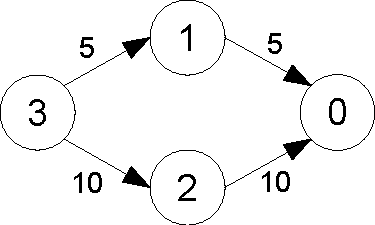
\includegraphics[width=0.5\hsize]{./5-idea/figs/motivationexample.pdf}
\end{center}
\caption{\textbf{Example routing problem.} The edges are the energy in mJ to
send a packet.}
\label{idea-fig-motivationexample}
\end{figure}

As a simple example demonstrating the need for IDEA, consider a four-node
routing problem. Figure~\ref{idea-fig-motivationexample} shows the network
topology, with the energy required to reliably transfer a packet over each
link shown. (To simplify the example we ignore receive costs, assume all
nodes have the same data rate of one packet per second, and assume a powered
sink.) The application attempts to localize events by collecting data from
all four nodes, meaning the loss of a single node will render the network
useless.

Node~3 has two routes to the sink Node 0: $3,1,0$ and $3,2,0$. If Node~3
conserves power by making a local greedy decision, it will route through
Node~1, since sending a packet to Node~1 consumes $0.5$~mJ of energy as
opposed to $1.0$~mJ for sending to Node~2. Even assuming Node~3 knows the
power consumption of the links $1,0$ and $2,0$, with no other information it
still chooses the route though Node~1, which consumes less total energy per
packet than the route through Node~2, 1.0~mJ per packet versus 2.0~mJ.

To facilitate our discussion we define $B_n$, $C_n$ and $L_n$ as the
battery in joules, charging rate in mJ per second, and non-routing load in mJ
per second at Node $n$ respectively.  $R^{Route}_n$ represents the cost to
Node $n$ assuming Node 3 uses the route indicated.  (Node~1 and Node~2 route
directly to the sink.) The choice we are considering is between two possible
load distributions, $R \in \mathcal{R}$, where:

\begin{itemize}

\item \textbf{$\mathbf{R^{3,1,0} = (0.0, 1.0, 1.0, 0.5)}$:} Node~1 uses 0.5~mJ sending
its own packet and 0.5~mJ routing for Node~3. Node~2 uses 1.0~mJ sending its
own packet. Node~3 uses 0.5~mJ sending its own packet to Node~1.
\vspace{-0.1in}
\item \textbf{$\mathbf{R^{3,2,0} = (0.0, 0.5, 2.0, 1.0)}$:} Node~1 uses 0.5~mJ
sending its own packet. Node~2 uses 1.0~mJ sending its own packet and 1.0~mJ
routing for Node~3. Node~3 uses 1.0~mJ sending its own packet to Node~2.

\end{itemize}

The question we ask is, under what conditions will using route $3,1,0$ ---
which consumes the least energy locally and globally --- actually
\textit{harm} application performance?  We identify four situations where
using the alternative route $3,2,0$ is the correct choice:

\begin{itemize}

\item \textbf{Differences in initial battery levels:} If the nodes are not
harvesting energy ($C_n = 0 \forall n$), no non-routing load exist ($L_n = 0
\forall n$), and Nodes~2 and~3 have significantly more energy than Node~1,
then routing through Node~2 will increase the lifetime of Node~1, which due
to its low battery level defines the lifetime of the network. Specifically,
if $B_2 > B_1 * 2$ and $B_3 > B_1 * 2$  then using $R^{3,2,0}$ will increase
the network's lifetime.

\item \textbf{Differences in non-routing load rates:} Assuming equal initial
energy availability and no harvesting, consideration of non-routing load
$L_n$ is similar to differences in battery sizes. Differences in non-routing
load rates between the nodes could be due to higher sampling rates or sensor
energy costs on various nodes. Assuming $B_n = \beta$ $\forall n$ and $C_n =
0$ $\forall n$, the result is similar: if $L_2 + 1.0 \le L_1 - 0.5$ and $L_3
+ 0.5 \le L_1 - 0.5$ then using $R^{3,2,0}$ will increase the network's
lifetime.

\item \textbf{Differences in charging rates:} If $C = [0.0, 2.0, 2.0, 2.0]$,
then both routes allow all nodes to continue to charge, but $R^{3,1,0}$ leads
to an aggregate charging rate of $4.0$~mJ/s whereas $R^{3,2,0}$ produces an
aggregate charging rate of only $2.5$~mJ/s, leaving $R^{3,1,0}$ the better
option. However, if $C = [0.0, 0.5, 2.0, 2.0]$, then the application must
choose between the lower aggregate charging rate of $1.5$~mJ/s but better
survivability of $R^{3,2,0}$ and the higher aggregate charging rate of
$2.5$~mJ/s but unsustainability of $R^{3,1,0}$. Since our application cannot
lose a single node, it chooses the lifetime of Node~1 over charging at
Nodes~2 and~3, and thus $R^{3,2,0}$. Note that if $C = [0, 0.5, 1.0, 1.0]$,
then no $R \in \mathcal{R}$ leads to a non-zero charging rate and the best
route is $R^{3,1,0}$.

\vfill\eject

\item \textbf{Overcharging:} Assuming that the batteries at Nodes~2 and~3
have reached capacity, but Node~1 has not, if $R^{3,2,0}_2 > C_2$ and
$R^{3,2,0}_3 > C_3$ then using $R^{3,2,0}$ will either increase the charging
rate at Node 1, if it is charging, or increase its lifetime by reducing its
load if it is not. Either outcome is beneficial.

\end{itemize}

Making the correct decision at Node~3 in all four cases requires that it know
the load rates, charging rates, and battery levels at Nodes~1 and~2. IDEA
addresses this problem by distributing this information across the set of
affected nodes. The four cases above motivate several features in the IDEA
design. In general, the network may want to shift load \textit{towards} nodes
that have a great deal of stored energy, low load rates, high charging rates,
or charging energy currently going to waste, and \textit{away} from nodes
with low batteries, low charging rates, or that are already highly-loaded. In
cases where shifting load produces extra overall load for the network, as it
does above, changes in load distribution must be managed by the application
based on its own goals and requirements. Had our application above been able
to tolerate the loss of Node~1, it might have chosen to optimize charging at
Nodes~2 and~3 in the third example. Respecting these differences, IDEA is
designed to incorporate application-level input into its decision-making
process.

\section{Lance System Architecture}
\label{lance-sec-architecture}

\begin{figure}[t]
\label{lance-fig-architecture}
\begin{center}
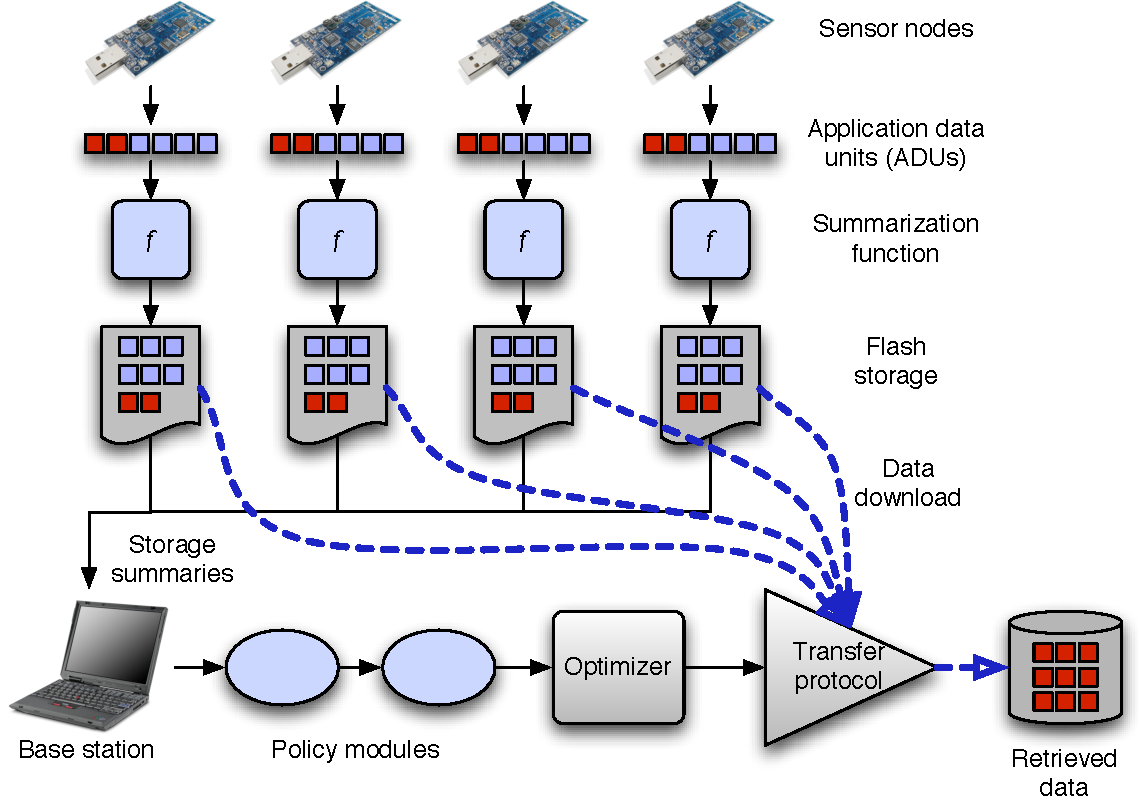
\includegraphics[width=1.0\hsize]{./4-lance/figs/new-arch.pdf}
\end{center}
\caption{\textbf{The Lance system architecture.}
The summarization portions are provided by the application; all other
components are generic.}
\end{figure}

This section describes the Lance architecture, introducing a
formal problem definition, design principles, and major system components.
Section~\ref{lance-sec-implementation} covers implementation details omitted here.

\subsection{Problem definition}
\label{lance-sec-problem-definition}

In Lance, the network consists of a set of sensor nodes that continuously
sample and store sensor data into {\em application data units (ADUs)}, which
are the unit of data storage and retrieval.  Each unique ADU $a_i$ consists
of a tuple $\{ i, n_i, t_i, d_i, v_i, \bar{c}_i \}$, 
where $i$ is a unique ADU identifier,
$n_i$ is the node storing the ADU, $t_i$ is a timestamp, and $d_i$ is the raw
sensor data.  We assume that ADUs are of uniform size and that nodes 
have sufficient flash storage to buffer collected signals, so an 
ADU is only evicted from a node's flash once it has been downloaded.
We define the {\em universe} $U$ as the set of all ADUs sampled by the 
network over time. 

Every ADU is assigned an application-specific {\em value} $v_i$ that
represents the application's intrinsic ``utility'' for the data contained
within the ADU.  We make no assumptions about how ADU values are assigned;
the value could be a function of the data itself, the time the data was
acquired, which node sampled the data, data being sampled by other nodes,
and so forth. Lance provides a flexible infrastructure for applications
to define their own value functions through policy modules.

Each ADU has an associated cost $\bar{c}_i$ that represents the energy
requirement to download the ADU from the network.  $\bar{c}_i$ is a vector
$\{ c_i^1, c_i^2, \ldots, c_i^n \}$ where $c_i^j$ represents the estimated
energy expenditure of node $j$ when ADU $i$ is retrieved. The key idea is
that we explicitly model both the energy cost for downloading the ADU from
its ``host'' node $n_i$ and the energy cost for each node along the
routing path from $n_i$ to the base station which must forward packets during
the transfer. In addition, we also model the energy cost to nodes that
overhear transmissions by nodes participating in the transfer.  This energy
cost on intermediate nodes is non-negligible, since reliable transfer
protocols involve a potentially large number of retransmission. However, the
overhearing cost is typically small, since modern low-power MAC protocols
quickly return to sleep when overhearing transmissions to another node.  The
cost vector $\bar{c}_i$ therefore depends on the network topology.

We assume that each node has a battery with a fixed capacity of $C$
joules, and no energy harvesting is performed in the field. 
Without loss of generality, let us assume that $C$ is
identical for all nodes in the network and is known {\em a priori}. 
We define the {\em lifetime target} $L$ as the desired lifetime 
of each node in the network. To meet the lifetime
target, nodes should strive to consume no more than $C/L$ 
joules per unit time on average; we call this the {\em discharge rate} of 
the node. 

The high-level goal of Lance is to download the set of ADUs that
maximizes the total value, subject to the lifetime target. Abstractly,
we define an {\em epoch duration} $\Delta$. Over each epoch, the 
energy consumption of each node must be less than the discharge rate,
that is, $\sum_i \sum_j c_i^j \leq \Delta \times C/L$. 
Determining the optimal set of ADUs to download can be determined by 
solving a multidimensional knapsack problem in which each ADU
represents an item to place in the knapsack with value $v_i$ and 
cost $\bar{c}_i$. The knapsack has $N$ dimensions (where $N$ is the
number of nodes in the network), each of size $\Delta \times C/L$
representing the energy availability over an epoch.
However, calculating the optimal
solution requires {\em a priori} knowledge of all ADUs generated by
the network over time. Clearly, any real system must make use of an
online, heuristic algorithm to approximate the optimal solution.
We discuss and evaluate several different approaches, presenting 
results with respect to the optimal offline solution.

\subsection{Design principles}

Before describing Lance in detail, we first outline several principles 
that guide its design. 

{\em Decouple mechanism from policy.}
We wish to make it easy to adapt Lance to different application
domains by providing a simple set of underlying mechanisms for 
weighing cost and data value that can be tailored 
for different
end-user goals. These core mechanisms should not be tied to any
interpretation of the data stored in an ADU. This approach leads 
to a clean separation of concerns between Lance's resource management
layer and the higher-level policies informing its operation.

{\em Simplicity through centralized control.} In a field deployment setting, 
it is highly desirable for the sensor network to be as simple
as possible, to prevent failures or unexpected behavior due to bugs.
Past deployment experiences have taught us, and others, that 
introducing complex dynamics within the network can lead to a system
that is difficult to understand, debug, or fix in the
field~\cite{volcano-osdi06,volcano-ewsn05}.
To maximize the chances of a successful deployment, 
Lance places most of the control
logic at the base station, treating sensor nodes as slave devices.
This principle makes it easy to change the behavior of the network
at the base station and allows nodes to fail independently without 
affecting the rest of the system. Conventional replication and
failover techniques can be used to bolster the reliability of the 
base station itself.

{\em Low cost for maintenance traffic.} Given limited node energy, 
we wish to reserve as much capacity as possible to support
data collection. This implies that the system
should strive to limit control messages between the base station and
the sensor nodes, as well as internal traffic within the network, as
transmitting packets unnecessarily consumes valuable energy.
This is somewhat at odds with the need for central control,
as the latter could require extensive coordination between 
sensor nodes and the base station; we wish to strike a good balance
between these two conflicting goals.

\subsection{System overview}

Figure~\ref{lance-fig-architecture} provides an overview of the Lance
architecture. Sensor nodes sample sensor data, storing the
data to local flash storage. Each application data unit (ADU)
consists of
some amount of raw sensor data, a unique {\em ADU identifier}, and a 
{\em timestamp} indicating the time that the first sample in the ADU
was sampled. ADU timestamps can either be based on local clocks at
each node, or tied to a global timebase using a time synchronization
protocol such as FTSP~\cite{ftsp}. The size of an ADU should be
chosen to balance the granularity of data storage and download with
the overhead for maintaining the per-ADU metadata. In the applications
we have studied, an ADU stores several seconds or minutes 
of sensor data, not an individual sample. ADUs are stored
locally in flash, which is treated as a circular buffer.

Ideally, nodes would be able to compute the value $v_i$ of an ADU
locally, as the data is sampled. However, since the value might depend
on factors other than the ADU's data, such as data computed at
other nodes. Lance assigns values $v_i$ at the base station,
based on global knowledge of the state of the network. However, this
requires nodes to communicate some low-bandwidth information on the ADU
contents to the base station.  For this purpose, each node applies an
application-supplied {\em summarization function}, computing a 
concise summary $s_i$ of the contents of the ADU as it is sampled.
Nodes periodically send {\em ADU summary} messages to the
base station, providing information on the ADUs they have sampled,
their summaries, timestamps, and other metadata. As a special case,
if a node is able to assign the ADU's initial value directly, this is used
as the summary.

The Lance {\em controller} receives ADU summaries from the network.
The controller also estimates the download cost $\bar{c}_i$ for each
ADU, based on information on network topology as well as a model of
energy consumption for download operations. The ADU summaries and cost
are passed through a series of {\em policy modules}, which provide
application-specific logic to assign the value $v_i$ to each ADU.
The resulting values are passed to the Lance {\em download manager}
which is responsible for performing downloads, using a reliable
data-collection protocol, such as Flush~\cite{flush-sensys07}.

\subsection{Summarization functions}

Lance computes ADU values using two application-provided components.  The
first is the summarization function, described above.  The second component
is a chain of {\em policy modules} executed at the base station which, by
modifying the value for each ADU, can implement a range of
application-specific policies. Since the base station receives ADU summaries
from every node, the policy modules can use global information not available
to individual nodes to make informed bandwidth and energy allocation
decisions.

Lance places two constraints on the on the summarization function. First,
we require that the summary be small (typically a few bytes) to limit the 
overhead for storing and transmitting these values. Second, 
the function must be able to run efficiently on the sensor node as 
ADUs are being sampled.  Otherwise, the exact form of the function is 
entirely application-specific.

As a concrete example, consider a network for downloading seismic events
from an earthquake zone.  One commonly-used measure of
overall seismicity during a time period is the Real-Time Seismic Amplitude
Measurement (RSAM)~\cite{rsam}, which computes the average amplitude
of a seismic signal over some time window (typically 1~to~10~minutes).
This function is simple to compute and reduces a complex seismic waveform
to a single scalar value, with higher values indicating greater seismic
activity.

Another form of summarization is an event detector, which would
produce a nonzero value whenever an event of interest is
contained within the ADU; the summary might also represent the strength
or confidence of the event detection. For example, an acoustic animal
tracking system~\cite{girod-ipsn07} or countersniper localization
system~\cite{shooter-localization} might use a simple trigger-based
summarization function, indicating the detection of a marmot call or
gunshot in the ADU.

\subsection{Cost estimation}
\label{lance-sec-costassignment}

Lance estimates the download energy cost
vector $\bar{c}_i$ for each ADU sampled by the network. 
We assume that nodes are organized into a spanning tree topology
rooted at the base station. The cost is a function of many factors,
including the reliable transport protocol, each node's position 
in the routing tree, radio link quality characteristics, and the 
MAC protocol. 

Given the complex dynamics that can arise during a sensor network's
operation, we opt to use a simple conservative estimate of the energy cost to
download an ADU from a node. Our approach is based on an empirical model that
captures three primitive energy costs involved in downloading an ADU. The
first, $E_d$, represents the energy used to download an ADU from a given node
which includes the energy cost for reading data from flash and sending
multiple radio packets (including any retransmissions) to the next hop in the
routing tree.  The second, $E_r$, represents the energy cost at intermediate
nodes to forward messages during the ADU transfer. The third, $E_o$,
represents the energy cost to nodes that overhear transmissions during a
transfer.  For simplicity, we assume ADUs of fixed size and compute $E_d$,
$E_r$, and $E_o$ based on the time necessary to download an ADU from the
target node.

Using this simple model, we set the elements of the cost vector $\bar{c}_i$ 
as follows. $c_i^n = E_d$ for the node $n$ hosting the ADU, and 
$c_i^m = E_r$ for nodes $m$ along the routing path from
$n$ to the base station. We set $c_i^o = E_o$ for nodes that are
assumed to be within one radio hop of any of the nodes involved in
the transfer. Estimating $\bar{c}_i$ therefore requires
knowledge of the current routing topology. This information 
is readily available: the periodic summary messages, sent to the 
base station by every node, include the node's radio neighbors and 
parent in the routing tree. Cost vectors can be easily recomputed 
whenever the routing topology changes.

To ensure that all nodes meet the lifetime target $L$, Lance models the
energy availability at each node using a token bucket with depth $D$ and fill
rate $C/L$, corresponding to the mean discharge rate.  $D$ is determined by
the target lifetime $L$, the battery capacity $B$ and the background drain
rate $R$.  In general, $D = B - L*R$, so $D$ represents the energy remaining
after the node reserves enough to ensure it can meet its target lifetime at
the background level.

\subsection{Lance optimizer}
\label{lance-sec-lanceoptimizer}

The Lance optimizer is responsible for scheduling ADUs for download,
based on knowledge of the set of ADUs currently stored by the
network, their associated values, and costs. 
ADU download itself is accomplished using a reliable transfer protocol such as 
Fetch~\cite{volcano-osdi06} or Flush~\cite{flush-sensys07}. In our
design, Lance attempts to download a single ADU at a time, in 
order to prevent network congestion, although it may be possible to
download multiple ADUs simultaneously, depending on the network
topology. A download completes either when the entire ADU has been
received or a timeout occurs.

Lance's optimization process attempts to maximize the value of the ADUs
retrieved while adhering to the lifetime target $L$. In essence, we seek a
greedy heuristic approximation of the multidimensional knapsack solution that
would be used by an oracle with complete knowledge of the ADUs sampled by the
network over all time.  The optimizer first excludes ADUs that would involve
nodes without enough energy to perform a download.  That is, if the token
bucket for a given node $m$ has $E(m)$ joules, ADUs for which $E(m) < c_i^m$
are excluded from consideration.  Note that as the bucket fills, the ADU may
become available for download at a later time. We call these ADUs {\em
infeasible}, and the remaining {\em feasible}.

To determine the next ADU to download, the optimizer considers the 
value $v_i$ of each ADU and the its associated cost $\bar{c}_i$.
We consider three {\em scoring functions} that assign a 
download score to each feasible ADU; the ADU with the highest download score
is downloaded next. In the case of ties, an arbitrary ADU is chosen.

The first scoring function, {\em value-only}, simply downloads the feasible
ADU with the highest value $v_i$. Note that {\em value-only} will meet the
network's lifetime target (since only feasible ADUs are considered) but does
not rank ADUs according to cost.  The second scoring function, {\em
cost-total}, assigns the score $\hat{v}_i$ by scaling the value of the ADU by
its total cost: $\hat{v}_i = v_i / \sum_j c_i^j$. The feasible ADU with the
highest score is then downloaded from the network. This approach penalizes
ADUs stored deep in the routing tree, which have a higher overall cost than
those located near the base station. 

The third scoring function, {\em cost-bottleneck}, scales the ADU value $v_i$ 
by the cost to the node that is an energy bottleneck for downloading
this ADU. That is, let $b$ represent the node with the minimum value
of $E(b)$ such that $c_i^b > 0$. {\em cost-bottleneck} sets the score
$\hat{v}_i = v_i / c_i^b$. The intuition behind this scoring function is
that the most energy-constrained node should be considered when
scoring ADUs for download. We evaluate all three scoring functions in 
this paper and show that they yield very different results in terms
of spatial distribution and energy efficiency.


\section{Case Studies}
\label{idea-sec-casestudies}

Throughout the rest of the paper we demonstrate IDEA using two examples.
Section~\ref{idea-sec-evaluation} presents results demonstrating the
performance improvements that IDEA delivers for each application.

\subsection{Energy-Aware Routing}

The second example shows how to integrate IDEA with an existing routing
protocol, namely the Collection Tree Protocol (CTP)~\cite{ctp-sensys09}. CTP
is a spanning-tree routing protocol that is a standard component in
TinyOS~\cite{tinyos-asplos00}. In CTP, each node selects its parent in the
spanning tree based on the \textit{expected number of transmissions} (ETX) to
reach the sink. This is an additive metric intended to limit queue occupancy
at nodes along each routing path and maximize packet delivery rates. Although
ETX can be directly converted to an energy measure (assuming the energy costs
to transmit along a link are known), CTP does not explicitly consider energy
availability in its routing decisions.

We integrate IDEA with CTP to create \textit{ICTP}, an energy-aware
load-balancing routing protocol that combines the use of ETX with IDEA's
energy objective function. As described in
Section~\ref{idea-subsec-energyobjectivefunctions}, we parameterize the
tradeoff between pure ETX and pure energy objective using the weighting
factor $\alpha$. When $\alpha = 1$ the minimum ETX path is always used and
ICTP behaves identically to unmodified CTP. When $0 < \alpha < 1$, potential
parents with path ETX $<$ minimum ETX $\cdot \frac{1}{\alpha}$ will be
considered, with the one producing the best energy objective score chosen.
When $\alpha = 0$, ETX is not considered at all and parent selection is
performed entirely on the basis of energy. Hence, $\alpha$ indirectly
controls the degree of path stretch that is induced by energy awareness. 

In order to build routes, CTP must periodically broadcast the current parent
and ETX to neighboring nodes. ICTP adds additional information to these
broadcasts, specifically the \textit{expected power}, or \textit{EPX}, for
transmissions to the node's parent. This information increases the size of
the broadcast packet sent by ICTP slightly, but does not appreciably affect
the energy consumption of the protocol's own data sharing, since the cost to
transmit a packet using LPL is a function of the receiver's polling interval,
not the packet size.

The local state space $s_n = \left\{s_n^{p_1}, s_n^{p_2}, \ldots, s_n^{p_k}
\right\}$ is defined by the node $n$'s neighbors $p_n = \left\{p^1, p^2,
\ldots, p^k \right\}$, each of them a prospective parent. CTP uses four-bit
wireless link estimation~\cite{Fonseca07} to estimate the ETX to each
neighbor, which ICTP multiplies by the power-per transmission to produce the
EPX to each neighbor, $EPX(n, p_n^i)$. Through ICTP data dissemination node
$n$ also learns the EPX from each neighbor to their current parent,
$EPX(p_n^i, \textrm{parent}(p_n^i))$. We have modified CTP to measure the
traffic rate $\delta(n)$, which is the number of packets per given interval
that node $n$ is forwarding to the sink. This is a function of both its own
packet generation rate and of the traffic induced by nodes upstream that it
is routing for. Given these parameters the projected energy load vector
$\bar{L}(s_n^{p_i})$ has two components: $L_n = \textrm{EPX}(n, p_n^i) \cdot
\delta(n)$ and $L_{p_i} = \textrm{EPX}(p_n^i, \textrm{parent}(p_n^i)) \cdot
\delta(n)$. Based on this information, IDEA chooses the best neighbor as the
node's parent.

Depending on the energy objective function chosen ICTP responds to variations
in load and charging rates in different ways. For the following discussion we
assume that the application uses the \textit{maximize first-node lifetime}
objective function described in
Section~\ref{idea-subsec-energyobjectivefunctions}, and so is willing to
trade off reduced charging rates or lifetimes at nodes that are not the
network's lifetime bottleneck in order to increase the lifetime of the node
projected to die first. Routing trees by their very nature concentrate load
near the base station, which we assume is powered. Without considering
variances in non-routing load or charging rates ICTP will attempt to balance
load across nodes that can communicate directly with the base station,
arranging the routing tree considering both the number of nodes upstream from
each of the base station's neighbors and the quality of their link to the
base station.

ICTP also responds to spatial variations in charging rates by building a tree
that is sensitive to where in the network energy is available. ICTP will
route around shadows in the network, or build routing backbones using
quickly-charging nodes or nodes whose batteries are full while attempting to
push nodes low on batteries into leaf roles, reducing or eliminating their
routing responsibilities.

Because ICTP reacts to changes in energy available by potentially choosing
routes with larger ETX, small values of $\alpha$ can begin to effect the
achieved packet delivery rate. We were able to find values of $\alpha$ that
produced significant performance improvements while leaving the delivery rate
unaltered. CTP has a persistent retransmission policy which assists us in
achieving good performance.

\subsection{Distributed Localization}

The third case study illustrates how to use IDEA to control discrete, rather
than continuous, network behavior. We consider a system designed to perform
acoustic source localization. Several previous systems have explored this
application in different contexts, including urban sniper
localization~\cite{shooter-localization} and localizing animals based on
mating calls~\cite{girod-marmots}. Using IDEA, it is possible to carefully
manage the energy load at each sensor node to prolong battery lifetime while
maintaining high localization accuracy.

Acoustic source localization involves calculating the location of an acoustic
source by collecting arrival times at several stations and performing a
back-azimuth computation. We assume a dense sensor network deployment, so
that an acoustic event is detected by many sensors. We also assume that for
each event, any set of four sensors that heard the event can correctly
perform the localization to within the application's error tolerance. 

A centralized approach to localization requires nodes to transmit data to a
base station where the computation is performed. Because we assume that nodes
cannot accurately compute an arrival time by only considering their own
sampled data, they must transmit a sizeable amount of data to the base
station to implement the centralized strategy, with the bulk data transfer
required producing a significant load on the nodes that heard the event as
well as nodes required to route data. This approach also does not scale well
as the size of the network increases.

To avoid the overheads of centralization we want to perform the localization
inside the network. However, the cost to transmit signals and perform the
computation are still high, so it is important that localization be done in a
way sensitive to the availability of energy within the network.

When an event occurs, the goal is to select a single \textit{aggregator} node
and three \textit{signal provider} nodes from the set of nodes that detected
the event. The signal providers will transmit a portion of the acoustic
signal to the aggregator, which performs the localization computation using a
time-of-arrival and angle-of-arrival computation~\cite{Niculescu03adhoc}.
For each event we expect multiple valid aggregator and signal provider sets
to exist, each with its own energy consumption signature. We refer to a
selection of four such nodes as a \textit{localization plan}. 

Nodes that heard the signal participate in a leader election process, seeded
by the value of the IDEA energy objective function for each proposed
localization plan. Each candidate aggregator computes the energy objective
function for the localization plan or plans that they are the aggregator for.
If more than three nodes within a single hop of an aggregator heard the
event, then the aggregator will have multiple plans to consider. The
aggregator chooses the local plan with the best score and broadcasts a
message advertising that score, which is propagated to all nodes that heard
the event. If the aggregator does not hear a broadcast with a better score,
it assumes that it won the leader election and proceeds to perform the
localization as planned. 

\section{Evaluation}
\label{idea-sec-evaluation}

To evaluate IDEA, we built and tested the energy-aware component and
application described in Section~\ref{idea-sec-casestudies}. For the routing
protocol, we compare our IDEA-based implementation to an approach that is not
energy-aware. For the application, we use IDEA to implement several energy
objective functions and compare their performance against each other and
against a heuristic that does not consider energy availability.

\subsection{Experimental Setup}
\label{idea-subsec-experimentalsetup}

Throughout the evaluation we present results run in several different
environments. We have implemented IDEA for TinyOS in order to run experiments
on MoteLab~\cite{motelab}, our 180~node wireless sensor network testbed. We
also present results obtained using TOSSIM~\cite{tossim}, the TinyOS
simulator. TOSSIM incorporates a closest-fit pattern matching noise model to
accurately capture complex link dynamics~\cite{cpm-ipsn07}. TOSSIM allows us
to run longer experiments incorporating various solar charging models. To
improve the realism of TOSSIM we began with a modified version developed for
the Koala project~\cite{koala-ipsn08} and performed further modifications to
correctly simulate the operation of low-power listening
(LPL), which is important to properly model the power
consumption of the radio for the ICTP experiments. We use information
collected on MoteLab to build a realistic TOSSIM radio model for our
simulations. Finally, for the application we built a Python simulator to
allow rapid prototyping of various energy objective functions.

IDEA is designed to tune components in the face of variations in both load
and charging rates, and to test this we present experiments using solar
charging data collected off of a solar panel deployed on an Arlington, MA
rooftop in March, 2009. Battery levels are calculated using a charging model
based on a Nickel-Metal Hydride battery technology with a 66\% charging
efficiency. We attenuate this data to simulate the charging produced by solar
panels of several different sizes in order to evaluate IDEA's performance as
available energy changes. We also perform experiments with a randomly
attenuated charging profile to simulate bad solar panel placement or
obstacles to incident sunlight effecting the spatial distribution of
collected energy.

For our MoteLab experiments we determine the system's ability to span periods
without charging inputs. We use two sets of initial conditions based on the
interaction between the charging data we collected and the capacity of the
batteries deployed. If the solar panel is large enough it will provide
considerable charging input and completely charge small batteries during the
day, so that all nodes begin the night with full batteries. If the solar
panel is not large enough to completely charge the batteries nodes will begin
the night with varying amounts of charge depending on their load rates during
the day.

Energy tracking is done by IDEA using a software-only approach developed for
the Pixie~\cite{pixie-sensys08} project. The component captures state
transitions and applies an energy consumption model for each state based on
current consumption measured offline. In the future we would like to
integrate a more accurate hardware-driven approach such as
iCount~\cite{icount-spots08}. The short lifetimes for some experiments are
explained by the use of extremely small batteries, which were chosen to allow
experiments to complete in reasonable amounts of time. We expect that
application developers will want to use a battery size and charging
technology suitable to allow their system to achieve a desired level of
performance, and the improvements in energy efficiency possible using IDEA
will allow smaller batteries or solar panels to be used, reducing the size
and cost of the hardware package.

Experiments for the energy-aware routing case use the first-node death energy
objective function described in
Section~\ref{idea-subsec-energyobjectivefunctions}, and therefore we evaluate
the network lifetime as the time at which the first node runs out of energy.
Our distributed localization application illustrates the process of designing
an effective energy objective function when the overall goal of the system is
known.

\subsection{ICTP: Energy-Aware Routing}

\begin{figure}[t]
\begin{center}
\textbf{(a)}\\
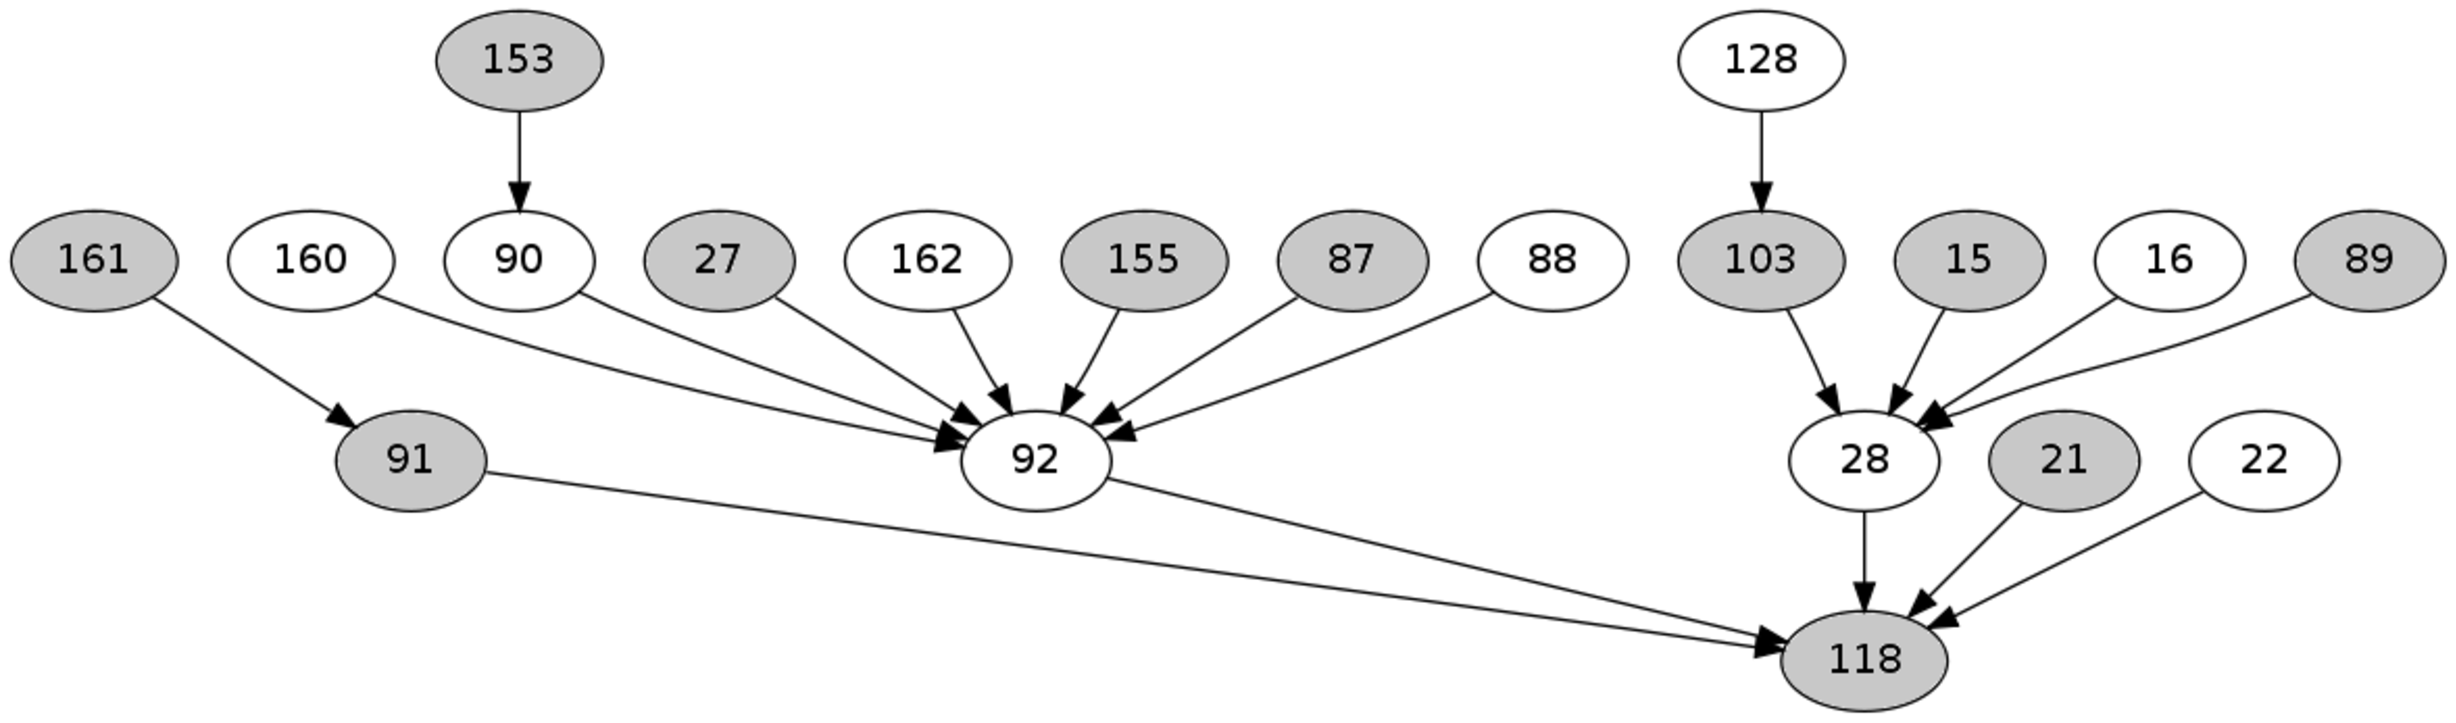
\includegraphics[width=0.7\hsize]{./5-idea/figs/ctp.pdf}\\
\textbf{(b)}\\
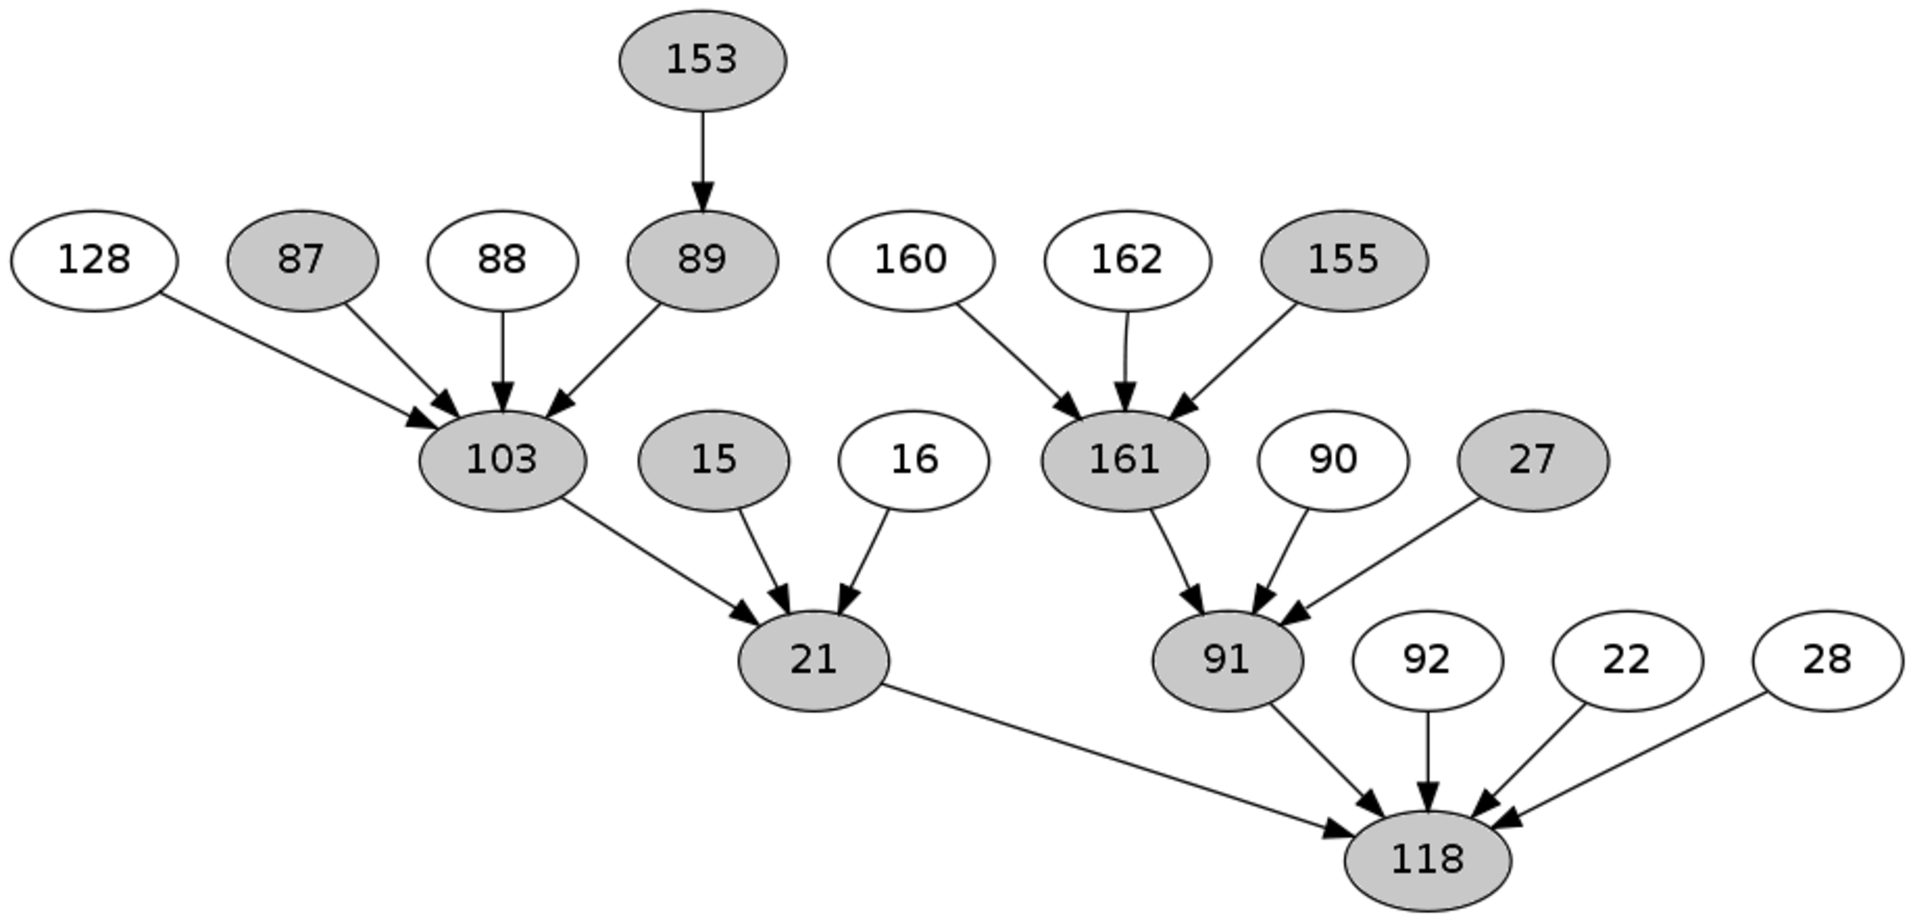
\includegraphics[width=0.7\hsize]{./5-idea/figs/ictp.pdf}\\
\end{center}

\caption{\textbf{Qualitative comparison of stock CTP and ICTP.} For this
experiment odd-numbered nodes (shaded) were set to charging rapidly, while
even-numbered nodes were not charging. Unmodified CTP builds the tree shown
in (a), which routes many packets through the even nodes. ICTP builds the
tree shown in (b), which moves all even nodes to leaf roles.}

\label{idea-fig-ictpqualitative}
\end{figure}

Using IDEA we were able to integrate energy awareness into CTP, the routing
protocol included as part of TinyOS. For these experiments each node in a
20~node network sends 6 packets to the sink per second. Static LPL intervals
of 0.5 second were used. 

Figure~\ref{idea-fig-ictpqualitative} shows a qualitative demonstration of
the difference between energy-aware and non-energy-aware routing trees. This
TOSSIM simulation ran with all odd numbered nodes charging rapidly and all
even numbered nodes not charging (with the exception of the powered sink,
Node 118). While this is an unrealistic charging pattern, it produces a clear
difference in routing protocol behavior.
Figure~\ref{idea-fig-ictpqualitative}(a) shows that unmodified CTP is unaware
of these charging differences and puts several even nodes, such as Node 92,
into positions where they are routing for multiple nodes. The total number of
nodes upstream from even numbered nodes in the stock CTP case is 14. In
contrast, ICTP realizes that the odd-numbered nodes have energy to spare and
the even-numbered nodes are lacking, and moves all even nodes to leaf roles.
None of the even nodes in Figure~\ref{idea-fig-ictpqualitative} are routing
data.

Using a 20~node subset of our MoteLab topology, we compared the performance
of ICTP to unmodified CTP using 24-hour TOSSIM simulations and the three
different solar charging scenarios previously described. As
Table~\ref{idea-table-ictpvoptimaltossim} shows, ICTP shows improvements in
lifetime over stock CTP of between 11 and 27\%. The different routing trees
formed by ICTP did not effect the packet delivery rates appreciably with the
largest change in packet delivery rate being 2.8\% (97.8\% for CTP vs. 95.0\%
for ICTP).

Finally, Table~\ref{idea-table-etxsearchradius} shows how IDEA can trade off
application utility with the energy objective function. The simulation
experiment uses a 25~node grid topology and, similar to the previous
experiment, half the nodes are charging rapidly while the other half are not.
Here our application-defined metric is expected transmissions to reach the
sink (ETX). A purely ETX-based tree will use the shortest route without
routing around the uncharging nodes, whereas an energy-aware tree will avoid
the uncharging nodes by constructing longer routes. We expect that,
prioritizing ETX will cause the total ETX of the entire tree --- defined as
the sum of the ETX of all the routes in use --- to decrease, while
prioritizing energy performance will cause the first-node lifetime of the
tree to increase.

Indeed, Table~\ref{idea-table-etxsearchradius} confirms this is the case. For
each experiment, we restrict the set of acceptable parents to be the minimum
available parent ETX plus an extra amount we call the ETX search margin. For
example, if the minimum available parent ETX is 5 and the ETX search margin
is 10, then we will consider all parents with ETX < 15. As the search margin
increases, IDEA will examine longer routes that may provide better energy
performance. As the table shows, increasing the ETX search margin leads to
longer average routes but also improves overall network lifetime.

\begin{table}[t]
\begin{center}
\begin{tabular}{|l|ccc|}
\hline
\textbf{Solar Charging} & \multicolumn{2}{c}{\textbf{Lifetime (hours)}} & \textbf{Increase} \\
\textbf{Pattern} & \textbf{CTP} & \textbf{ICTP} & \textbf{(\%)} \\ \hline
Large Panel & 17.1 & 19.0 & 11\% \\
Small Panel & 10.5 & 13.3 & 27\% \\
Random Attenuation & 10.5 & 12.2 & 16\% \\ \hline
\end{tabular}
\end{center}

\caption{\textbf{ICTP performance with solar charging.} The table summarizes
the performance improvements obtained by replacing CTP with ICTP. Three
different solar charging profiles are used: a large panel that completely
charges all batteries each day, a small panel that does not, and a randomly
attenuated charging profile that varies node-to-node.}

\label{idea-table-ictpvoptimaltossim}
\end{table}

\begin{table}[t]
\begin{center}
\begin{tabular}{|l|cc|}
\hline
\textbf{ETX Search} & \textbf{Total ETX} & \textbf{Network Lifetime} \\
\textbf{Margin (ETX)} & \textbf{(ETX)} & \textbf{(sec)} \\ \hline
0 & 2442 & 4357 \\
10 & 2591 & 4737 \\
20 & 3207 & 5116 \\
50 & 3127 & 6216 \\
100 & 3442 & 6502 \\ \hline
\end{tabular}
\end{center}

\caption{\textbf{Tradeoff between energy-awareness and application utility.}
The results illustrate how IDEA can parameterize the tradeoff between
application-defined utility and the energy objective function.}

\label{idea-table-etxsearchradius}
\end{table}

\subsection{Distributed Localization}

To evaluate the distributed localization application we built a Python
simulator, which improves significantly on TOSSIM performance for hundreds of
nodes and allowed rapid iteration and experimentation with different energy
objective functions. Our simulator models acoustic event sources within the
sensor network, each of which triggers a distributed localization operation.
The energy overheads of communication, both the leader election process and
the subsequent data transfer, are modeled in the simulator based on empirical
measurements taken on our MoteLab testbed.

\begin{figure}[t]
\begin{center}
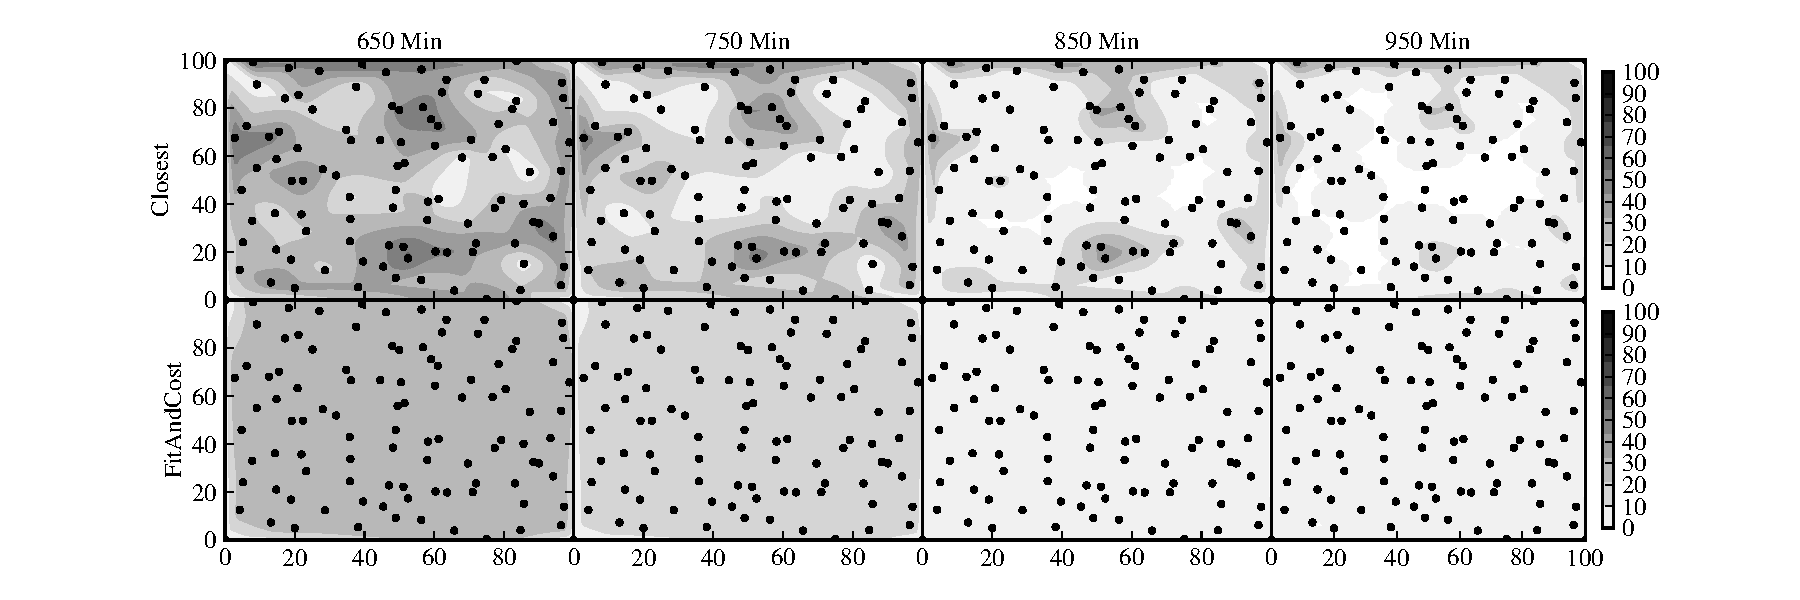
\includegraphics[width=\hsize]{./5-idea/figs/localizationdensityvtime.pdf}
\end{center}

\caption{\textbf{Energy density over time.} Energy densities for the
\texttt{Closest} heuristic and IDEA using the \texttt{WeightedEnergy}
objective function are shown at four points in time. The event distribution
is uniform. IDEA enables better load distribution, which leads to a longer
application lifetime.}

\label{idea-fig-localizationdensityvtime}
\end{figure}

For these experiments we arranged 100 nodes into a 100~m by 100~m area,
resulting in the placements shown in
Figure~\ref{idea-fig-localizationdensityvtime}. We simulate a sensing range
equal to the communication range, each set to 20~m. This radius is chosen to
give each node reasonable number of neighbors and allow it to detect a
reasonable number of events. We randomize the reliable transfer protocol
bandwidth across each link to between 768 and 1280~bytes/sec, a feasible
range based on results from data transfer protocols such as
Flush~\cite{flush-sensys07} and Fetch. Events are simulated using a uniform
random distribution so that events have equal probability of occurring
anywhere in the sensor field.

To evaluate network performance, we define \textit{capability} of the network
as the percent of the last 100 operations that succeeded, where success is
defined as localizing the event. We assume that the application requires that
the network be able to be able to localize a high percentage of events that
occur, and design our energy objective functions with this in mind. As an
example, an intruder localization application is no longer useful once it
fails to detect a very high percentage of intrusion attempts. We quote the
system lifetime as the the 90\% capability time, the time at which the
network's capability drops below 90\%.

We experimented with several approaches to choosing a localization plan, one
that does not use IDEA and three that do using different energy objective
functions:

\begin{enumerate}

\item \textbf{\texttt{Closest}:} produces a localization plan with the node
closest to the event source as the aggregator and the three next closest
nodes as signal providers. We assume a real solution would use an imperfect
estimate of proximity such as total signal energy or signal-to-noise ratio,
but for the simulations we use the known simulated event location to choose
the closest nodes. \texttt{Closest} does not require energy state information
and so could be implemented without IDEA. It is implemented as an example of
a plausible non-energy-aware solution.

\item \textbf{\texttt{MaxEnergy}:} chooses the node with the most energy
(that heard the event) as aggregator and the next three highest-energy nodes
as signal providers.

\item \textbf{\texttt{TotalEnergy}:} chooses the localization plan that
consumes the lowest amount of total energy summed across all nodes in the
network.

\item \textbf{\texttt{WeightedEnergy}:} weights the total energy consumption
using a similarity metric derived from the cosine similarity index to measure
the degree to which the energy vector for the localization plan is a good
``fit'' given the current energy availability.

\end{enumerate}

\begin{figure}[t]
\begin{center}
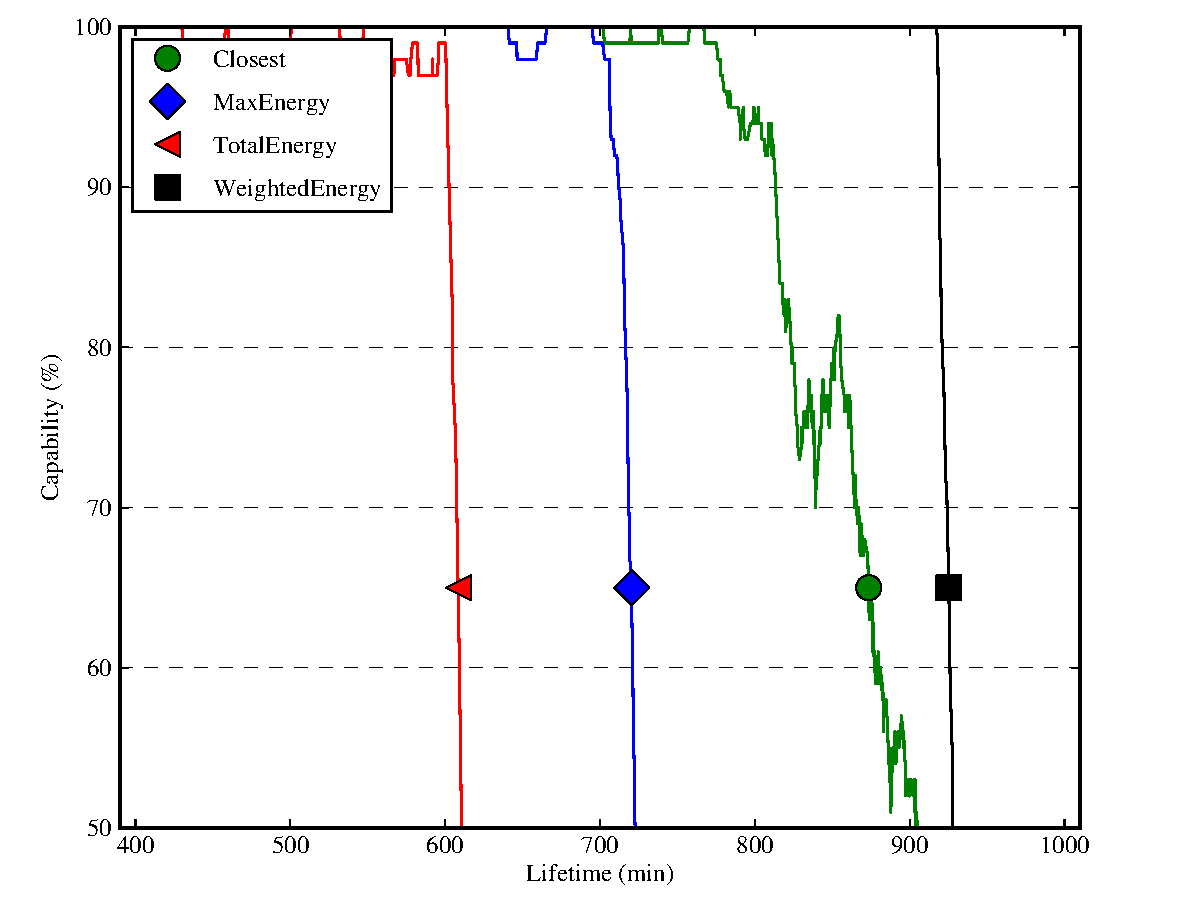
\includegraphics[width=0.7\hsize]{./5-idea/figs/ideavheuristics.pdf}
\end{center}

\caption{\textbf{Performance of IDEA objective functions and heuristic.}
Simulation results are shown for the localization application. The graph
compares the \texttt{Closest} heuristic, implemented without using IDEA,
against three different IDEA objective functions: \texttt{MaxEnergy},
\texttt{TotalEnergy} and \texttt{WeightedEnergy}. The \texttt{WeightedEnergy}
approach using IDEA outperforms the non-energy-aware approach while the other
objective functions perform more poorly.}

\label{idea-fig-ideavheuristics}
\end{figure}

We began by experimenting with the \texttt{Closest}, \texttt{MaxEnergy} and
\texttt{TotalEnergy} approaches. As Figure~\ref{idea-fig-ideavheuristics}
shows, the \texttt{Closest} heuristic outperformed the two IDEA-based
approaches. However, when examining the energy density plot shown in
Figure~\ref{idea-fig-localizationdensityvtime} for the \texttt{Closest}
heuristic we could see that it led to concentrations of available energy on
nodes at dense locations on the irregular grid, while \texttt{MaxEnergy} did
a better job of exhausting all nodes simultaneously, as evidenced by the
extremely sharp drop in network capability it produces. This is despite the
uniform distribution of acoustic event sources, which one might expect to
produce good energy load distribution without the need for tuning.

Our analysis determined that the \texttt{MaxEnergy} suffers because it will
always route data through extra nodes in order to reach the node with the
most energy. So if that node is on the edge of the cluster of nodes that
heard the event, energy may be consumed by nodes within the interior in order
to allow the signal provides to communicate with the aggregator.
\texttt{MaxEnergy} leads to an even usage of energy across the network, but a
short lifetime, because it always prioritizes the distribution of energy over
the amount consumed when choosing how to localize each event.

In contrast, \texttt{Closest}, while it performs better, has the opposite
problem. While it does not consider energy directly, the effect of the
heuristic is to choose based on the total amount of energy consumed. By
selecting the nodes closest to the event, the heuristic almost always leads
to clusters where all signal providers can communicate with the aggregator,
so no extra energy expenditures by other nodes for routing are needed.
However, the non-uniform distribution of nodes means that some nodes more
likely to be the closest node than others, leading to unequal energy
distribution. While the lifetime is better than \texttt{MaxEnergy}, the
existence of energy at some nodes once the capability drops below 90\% led us
to believe that a hybrid approach was possible that would outperform both
\texttt{MaxEnergy} and \texttt{Closest}.

After exploring several additional approaches we found an energy objective
function capable of producing extremely good load distribution, the
\texttt{WeightedEnergy} approach described above.
Figure~\ref{idea-fig-ideavheuristics} shows that it outperforms
\texttt{Closest}, increasing the network's lifetime by 15\%, while
Figure~\ref{idea-fig-localizationdensityvtime} illustrates how it utilizes
all the nodes' available energy, achieving an even distribution similar to
\texttt{MaxEnergy}. It does this by combining aspects of both earlier
approaches. By weighing the total energy consumed it avoids the extremely
high-energy localization plans that the \texttt{MaxEnergy} function will
sometimes use. By also weighing the ``fit'' using the cosine similarity
metric we address unequal energy distribution in a way that the
\texttt{Closest} heuristic does not.

Our experience with the localization application illustrates the role of the
proper energy objective function in enabling good application performance,
and points to the increases in system lifetime possible through better energy
distribution. 

\section{Related Work}
\label{sec-relatedwork}

This section discusses four kinds of related systems, those designed to cope
with high data rates, designed to operate in scientific contexts, and related
to Lance or IDEA.

\subsection{High Data Rate Sensing}

Many sensor network applications require collecting high-resolution signals
using low-power nodes. Examples include monitoring acoustic, seismic, and
vibration waveforms in bridges, industrial equipment, and animal habitats.
These systems all attempt to acquire high data rate (100~Hz or higher),
high-fidelity data across the network subject to severe constraints on radio
bandwidth and energy usage.

A group from UC Berkeley performed the largest deployment to date of sensor
network nodes for structural health monitoring: 46 nodes placed on the Golden
Gate Bridge~\cite{ggb-ipsn07}. Nodes collect vibration data at 1~kHz, and the
network uses many of the same routing and time synchronization protocols used
by our volcano monitoring system. A special bulk data collection protocol,
called Straw, was developed for the deployment. The highly linear topology of
the deployed network was later used to test the Flush data collection
protocol~\cite{flush-sensys07}. The deployment at the Golden Gate Bridge also
gave rise to a system called the Structural Health Monitoring Toolkit
(Sentri) that interfaces between the outside world and the sensor network by
transmitting commands to nodes as necessary.

NetSHMis a wireless sensor network for structural health monitoring, which
involves studying the response of buildings, bridges, and other structures to
localize structural damage, e.g., following an
earthquake~\cite{netshm-ewsnsubmission,netshm-emnets05,wisan}. This system
shares many of the challenges of geophysical monitoring. Indeed, the data
rates involved (500~Hz per channel) are higher than are typically used in
volcano studies. The Wireless Modular Monitoring System (WiMMS) is another
structural monitoring network with similar goals that has been validated both
in field deployments at the Geumdang Bridge in Icheon, South Korea, and in
laboratory tests~\cite{wimms-lynch06}. This system is designed to supporting
decentralize control algorithm that respond to structural changes using
actuators. In this context decentralization reduces the amount of data that
must be transmitted to a central location while eliminating the base station
as a single point of failure.

NetSHM implements reliable data collection using both hop-by-hop caching and
end-to-end retransmissions. The work explores the use of local computations
on sensors to reduce bandwidth requirements. Rather than a global
time synchronization protocol, the base station timestamps each sample upon
reception. The \textit{residence time} of each sample as it flows from sensor
to base is calculated based on measurements at each transmission hop and used
to deduce the original sample time.

Several factors distinguish our work on volcano science from structural
monitoring applications. First, structural monitoring networks typically
either collect data following controlled excitations of a structure or at
periodic intervals, which simplifies transmission scheduling. In our case,
volcanic activity is bursty and highly variable, requiring more sophisticated
approaches to event detection and data transfer. While the Golden Gate Bridge
system is sparsely deployed like our volcano sensor networks, many structural
monitoring applications are deployed in relatively dense networks, making
data collection and time synchronization more robust. 

Condition-based maintenance is another emerging area for wireless sensor
networks. The typical approach is to collect vibration waveforms from
equipment (e.g., chillers, pumps, etc.) and perform time- and
frequency-domain analysis to determine when the equipment requires servicing.
Intel Research has explored this area through deployments at a fabrication
plant and an oil tanker in the North Sea~\cite{intel-northseasensys}.
Although this application involves high sampling rates, it does not
necessarily require time synchronization as signals from multiple sensors
need not be correlated. The initial evaluation of these deployments only
considers the network performance and does not address data fidelity issues.

While many early environmental monitoring applications are characterized by
low data rates, some have focused on applications requiring high-speed data
acquisition. An example application is monitoring colonies of marmots. A
group at MIT led by Lew Girod has explored several generations of hardware
and software solutions for distributed acoustic monitoring driven by this
application~\cite{girod-marmots}. This work produced the Acoustic
ENSBox~\cite{girod-ensbox}, a self-calibrating hardware solution designed to
be easy to deploy in support of acoustic sensing applications. The ENSBox
features an ARM processor, which puts it at a different point on the
power-performance curve from typical sensor network nodes and makes it more
suitable for the high-speed processing necessary to capture acoustic signals.

The software environment for the ENSBox was originally provided by
EmStar~\cite{emstar}, which targets Linux-based platforms. More recently, the
ENSBox has been used as the basis of the VoxNet platform, an environment
designed for acoustic signal collection and processing.
VoxNet~\cite{voxnet-ipsn08} is comprised of three pieces:
Wavescope~\cite{wavescope}, a programming environment targeting
heterogeneous sensor networks. Wavescope programs are written in
WaveScript~\cite{wavescript-techreport08}, a stream-processing language.
Users compose a set of filters and other stream operators into a ``script''
similar to a data-flow graph.

The VoxNet platform includes a variety of network services, such as
time synchronization, routing, and node localization that applications
running in this environment can make use of. Once the program is written and
installed on nodes, VoxNet includes a set of control and visualization tools
intended to allow users to interact with the running system and view the data
as it is collected. A system using VoxNet was deployed in 2008 at the Rocky
Mountain Biological Laboratory and used to study the alarm calls of marmots.
Acoustic monitoring has scientific applications to other species as well, as
a variety of animals and birds produce scientifically-interesting
vocalizations.

Another application of high data rate sensing to habitat monitoring is the
cane toad monitoring project run by a team at Portland State University,
CSIRO, and the University of New South Wales. The cane toad is an invasive
species in Australia, and their spread is being monitored due to concerns
about their impact on the country's native fauna. The goals of the project
are to design a system permitting \textit{in situ} classification of various
frog species based on their vocalizations.

After completing a pilot study, two additional iterations advanced the design
of the system. In the first, a hybrid network was developed, mating low-power
sensor nodes and middle-tier devices with more advanced processing and
storage capabilities. Data reduction is performed on the sensor nodes in
order to limit the amount of information that must be sent to the high-power
devices, thus prolonging the lifetime of the embedded
nodes~\cite{canetoad-tosn}. The second iteration explores compressive
sampling techniques and also deploys a classification algorithm that can be
run directly on the resource-constrained sensor nodes.

Camera-based sensor networks also produce high data rates and have been the
subject of considerable study. A group at UCLA built a system called
Cyclops~\cite{cyclops-sensys05} which brings vision technology to sensor
network devices by offering a low-power imaging devices better suited to mating
with resource-constrained sensor nodes. They show that Cyclops nodes can
successfully perform fundamental vision-recognition tasks such as object
detection and hand posture recognition. Another team at UMass Amherst sees
motes fitted with imagers as forming one tier of a multi-tier multi-modal
($M^2$) sensor network~\cite{m2-nossdav05}. Such $M^2$ networks consist of
several tiers operating at different power levels while attempting to combine
the capabilities of multiple types of devices. The lowest tier might consist of
low-power sensor nodes equipped with vibration sensors and be used to trigger
the operation of more power-hungry devices --- such as
Stargates~\cite{stargate} fitted with webcams --- in the upper tiers.

\subsection{Scientific Sensing}

The first generation of sensor network deployments focused on distributed
monitoring of environmental conditions. Representative projects include the
Great Duck Island~\cite{spm:04habitat,polastre-masters,mainwaring-habitat},
Berkeley Redwood Forest~\cite{berkeley-redwoods}, and James
Reserve~\cite{cerpa-habitat} deployments. These systems are characterized by
low data rates (sampling intervals on the order of minutes) and very
low-duty-cycle operation to conserve power. Research in this area has made
valuable contributions in establishing sensor networks as a viable platform
for scientific monitoring and developing essential components used in our
work. 

This previous work has not yet focused on the efficacy of a sensor network as
a scientific instrument. The best example is the Berkeley Redwood Forest
deployment~\cite{berkeley-redwoods}, which involved 33~nodes monitoring the
microclimate of a redwood tree for 44~days. Their study focuses on novel ways
of visualizing and presenting the data captured by the sensor network, as
well as on the data yield of the system. The authors show that the
microclimactic measurements are consistent with existing models, but ground
truth of the data is not established. This paper does highlight many of the
challenges involved in using wireless sensors to augment or replace existing
scientific instrumentation.

A group at UCLA has built a system for soil monitoring and deployed it in the
AMARSS transect in the James Reserve, a biological field station operated by
the University of California. The goal was to augment a set of wired data
loggers with wireless sensor technology, similar in spirit to what we have
attempted with our volcano monitoring system. Since 2005 the deployed system
has collected over 26~million measurements, which are retrieved periodically
by a technician visiting the deployment site. The goal is to study the carbon
cycle and estimate the flux of carbon dioxide from the soil.

The largest challenge facing these researchers was coping with missing data.
To address it, they built a system called Suelo~\cite{suelo-sensys09}.  Suelo
is intended to aid human researchers in monitoring and assisting the health
of the deployment, sense the soil-monitoring sensors used are quite fragile.
Suelo monitors the readings capture by the network and tries to distinguish
between ``interesting'' and ``faulty'' data, and initiating human
intervention when sensors require replacement or recalibration.

Computer scientists at UMass Amherst have been deploying GPS-enabled sensors
to study the movement of a threatened species of turtle. This work led to
Eon, a language and runtime system designed to enable energy-aware
programming. Eon claims to be the first energy-aware programming language and
tries to make resource usage explicit to programmers by allowing them to
annotate their code with energy states. At runtime, Eon will adapt the
behavior of the node based on resource availability.

Similar to our work in its application to environmental hazard mitigation,
previous projects have explored sensor networks for flood and landslide
detection, at MIT and John Hopkins University, respectively. The MIT system
feeds data from a network of sensors into a model designed to predict
rainfall-triggered flooding~\cite{basha-sensys08}. They were able to show the
demonstrate the accuracy of their approach using data collected over multiple
field deployments on Honduras between 2004 and 2007. JHU's approach to
landslide detection employs sensor columns, vertical underground
installations of several different sensors~\cite{landslide-sensys05}. When a
portion of the deployed network detects that a slip surface is forming, nodes
cooperate to estimate the position of the slip surface which is fed into a
model that predicts whether and when a landslide will occur. Both of these
projects differ from our work by involving significant modeling and
prediction components, whereas we have focused primarily on raw data
collection.

Of particular interest is ongoing work at Washington State University using
camera-dropped sensor networks to monitor the activity of Mt. St.
Helens~\cite{wsuvolcano-mobisys09}. This project shares many of our goals,
including ease of deployment and data fidelity, but differs in its focus on
system lifetimes of up to 1~year, and in its aim to replace, rather than
augment, existing volcano monitoring stations. The reliance on helicopter
support while deploying nodes also leads to a different set of design
decisions, including much larger batteries and more capable nodes.

The WSU group uses an iMote2~\cite{imote2} sensor node, which shares the
CC2420 802.15.4 radio with our TMote but features the PXA271 XScale processor
with significantly more computational horsepower than the MSP430. The
expanded form factor and power budget permits the use of GPS at each node,
simplifying time sychronization (although FTSP is available as a backup if
the GPS signal is lost).

While the system aims to provide continuous data collection, the limited
bandwidth of the 802.15.4 radios on each sensor node and the 900~MHz
Freewave~\cite{freewave} modem used to maintain a connection with the
observatory limit the data that can be collected. Similar to our
volcano-monitoring system, an impulse detector implemented as a short-term
average over long-term average (STA/LTA) is used to assign a priority to the
data as it is collected. Data prioritization is used during data collection
and routing to ensure that data from detected events reaches the observatory
first. Currently the system works around energy limitations by using heavy
AIR-ALKALINE batteries, which are feasible because the nodes are being
deployed by helicopter.

\subsection{Data Quality Optimization Frameworks}
\label{lance-sec-related}

Several systems are related to Lance but differ substantially in their goals
and assumptions.

EnviroMic~\cite{enviromic} is a system designed to support distributed
acoustic recording by leveraging the collective storage resources of multiple
sensor nodes. It performs cooperative recording by organizing nodes into
groups when multiple nodes detect the same acoustic event, and using these
groups to ensure that only one node is recording acoustic data for as long as
the event of interest continues. This is intended to reduce the amount of
data that must be stored by eliminating redundant signal collection.

EnviroMic also focuses on distributing the storage load within the network to
ensure that the distributed storage can be utilized and signals of interest
not lost due to full Flash drives. While nodes may exchange data to rebalance
storage during the experiment, the fundamental assumption of the architecture
is that data will be manually retrieved from sensor nodes following the
deployment. Unlike Lance, EnviroMic is not intended for applications with
real-time data needs.

ICEDB~\cite{zhang2007icedb} supplies a delay-tolerant and priority-driven
query processor for the CarTel~\cite{cartel} system. ICEDB provides SQL
extensions allowing queries to assign both inter- and intra-stream
priorities, which are used by the query processor to manage bandwidth and
storage resources. ICEDB also uses a similar node-level summarization
technique to that used by Lance.

While ICEDB considers bandwidth limitations, it does not consider energy as a
constraint. The fundamental goal of ICEDB --- to provide database-like access
to mobile nodes that may experience periods of disconnection or poor
connectivity --- differs from that of Lance, which explains the architectural
differences. CarTel nodes are much higher-power and assumed to be attached to
power sources in the vehicles that they are deployed in.

VanGo~\cite{vango} provides an architecture for collecting and processing
high-resolution sensor data on resource-constrained nodes. VanGo focuses on a
programming model based on a linear filter chain and implementing efficient
signal-processing operations with limited computational power.
WaveScope~\cite{wavescope} and Flask~\cite{flask-tr} are languages for stream
processing applications. These systems are largely complementary to Lance,
and could be used to process signal data prior to collection, although our
focus is on collecting \textit{raw} sensor data from large networks. These
systems do not attempt to optimize data collection under varying energy and
bandwidth constraints. 

\subsection{Energy Load-Balancing Services}
\label{idea-sec-related}

Previous work has addressed the problem of energy load balancing in contexts
such as sensor coverage, role assignment, and energy-aware routing. Other
efforts in sensor networks have focused on reducing the power consumption at
individual nodes without considering energy distribution. Many of these
efforts are specific to a particular application or component and do not
provide a service like IDEA that can be used by a variety of applications. 

A number of existing systems such as Odyssey~\cite{odyssey-osr99},
PowerScope~\cite{powerscope-wmcsa99} and more recently
Cinder~\cite{cinder-mobiheld09}, have addressed measuring or adapting to
energy variations on battery-powered devices, primarily to support mobile
applications. This naturally produces a difference in approach from IDEA,
since IDEA targets networks consisting of multiple nodes but treated as a
single entity. Since nodes are collaborating we can enable more sharing and
ask nodes to sacrifice for each other, whereas mobile device users would
likely be upset if they discovered that their phone was running low on power
because it was trying to improve the lifetime of a stranger's phone located
nearby.

Quanto~\cite{quanto-osdi08} provides a framework for tracking and
understanding energy consumption in embedded sensor systems. The existence of
systems such as Quanto was a primary motivation for IDEA, since the
visibility distributed resource tracking provides creates an opportunity to
adapt to changes in availability across the network. Currently IDEA requires
that components model their own energy consumption, which may be difficult
for components with complex behavior. We are exploring integrating Quanto
into IDEA to provide more precise tracking of energy at runtime, which could
eliminate the need for component-specific modeling and ease the process of
integrating applications with IDEA.

Eon~\cite{eon-sensys07} performs similar energy tracking and forward
projection but focuses on single-node, not network-wide adaptations.
SORA~\cite{sora-nsdi05} focuses on decentralized resource allocation based on
an economic model in which nodes respond to incentives to produce data or
perform specific tasks, with each node trying to maximize its profit for
taking a series of actions. While SORA, using correctly set prices, could
produce similar network-wide behavior to that enabled by IDEA, the connection
between prices and the behavior of the network is not completely clear. IDEA
simplifies the problem of global network control through the energy objective
function which encapsulates the application's goal.

Some work on energy-aware routing~\cite{ShahRabaey2002,381685} has addressed
equitable energy distribution within the network by probabilistically
choosing between multiple good paths between each source and sink pair.
LEACH~\cite{leach} and other similar approaches attempt to distributed energy
in an entirely decentralized way, using local heuristics to do so.
Lexicographically maximum rate allocation~\cite{fairrate-sensys08} uses a
decentralized algorithm to tune optimum data collection rates in perpetual
networks when static routes are used, all nodes route to a single sink, and
the recharging profiles of the nodes are known ahead of time. Rate allocation
could be implemented in IDEA and comparing the two is planned future work.

VigilNet~\cite{vigilnet} is a target-tracking system that attempts to save
energy by rotating ``sentry'' duties between a group of nearby nodes. Nodes
that are not assigned as sentries can sleep and conserve energy while the
sentry monitors the area. When an event occurs, the sentry awakes nearby
nodes and initiates the tracking process. VigilNet assigns sentry duties
based on each node's energy availability while trying to ensure that the
entire area being monitoring is covered. Given the desire both to extend
system lifetime and maintain a desired application fidelity, VigilNet could
be implemented using IDEA, allowing both energy availability and harvesting
to be considered when assigning setries.

EnviroMic~\cite{enviromic} is a distributed acoustic storage system for
sensor networks. When EnviroMic nodes hear an acoustic event, a leader is
elected to assign recording tasks to nodes in the group. As storage space is
limited, EnviroMic attempts to push data to quiet sections of the network
with unused storage, balancing storage consumption across the network. Both
of these tasks involve choosing from a set of nodes that can perform the same
storage task, and so EnviroMic could be integrated with IDEA allowing the
energy overheads of data transfers to be considered.

The IDEA architecture emerged from our own prior work on energy management
for wireless sensor networks, including Lance (Chapter~\ref{chapter-lance})
Pixie~\cite{pixie-sensys08}, and Peloton~\cite{peloton-hotos09}. Pixie
proposed an operating system and programming framework for sensor network
nodes that promotes resources to a first-class primitive, using tickets to
manage resource consumption and brokers to enable specialized management
policies. Pixie does not consider the energy impact of a node on other nodes.

Peloton proposed an architecture for distributed resource management in
sensor networks combining state sharing, vector tickets to represent
distributed resource consumption and a decentralized architecture in which
nodes serve as ticket agents managing the resource consumption of themselves
and on behalf of nearby nodes. IDEA shares many features with Peloton and can
be viewed as the beginnings of an implementation of the Peloton design, with
state sharing to enable energy decision making and every node serving as a
ticket agent for itself but considering the distributed impact of its own
local state.

\section{Future Work and Conclusions}
\label{idea-sec-futurework}

As future work we are interested in addressing the problem of cross-component
interaction to be able to optimize the operation of several IDEA components
running in the network simultaneously. This is complicated by the fact that
there is likely to be dependencies between components that cause decisions
made by one to affect others. As an example, the LPL intervals used by a node
would effect the power cost to use the link seen by the routing protocol.  In
addition we are investigating ways to model the impact of node failure on
other nodes. Many sensor network protocols will try to work around nodes
leaving the network or going offline, but this repair process is costly and
causes load within the network to shift.

To conclude, we have described the IDEA architecture in detail, motivated its
use through three examples, and demonstrated that for each example IDEA can
improve performance by better managing distributed energy resources. We have
also discussed the process of developing an application-specific energy
objective function and shown how this can improve the performance of a
localization application while maintaining application fidelity.
\vfill\eject


\begin{footnotesize}
\bibliographystyle{abbrv}
\bibliography{mobisys10}
\end{footnotesize}

\end{document}
